% begin module definite-integral-properties-comparison
\begin{frame}[t]
Comparison Properties of the Integral
\begin{enumerate}
\setcounter{enumi}{5}
\item  If $f(x)\geq 0$ for all $a\leq x \leq b$, then $\displaystyle \int_{a}^{b} f(x)\diff x \geq 0$.
\end{enumerate}
\end{frame}

\begin{frame}[t]
Comparison Properties of the Integral
\begin{enumerate}
\setcounter{enumi}{6}
\item  If $f(x)\leq g(x)$ for all $a\leq x \leq b$, then $\displaystyle \int_{a}^{b} f(x)\diff x \leq \int_{a}^{b} g(x)\diff x$.
\end{enumerate}
\begin{center}
\psset{xunit=0.9cm, yunit=0.9cm}
\begin{pspicture}(-5, -5)(5,5)
\psframe*[linecolor=white](-5,-5)(5,5)
\psaxes[ticks=none, labels=none]{<->}(0,0)(-0.5,-0.5)(6,4.5)\tiny
\rput[l](5.1, 2.6){$y=g(x)$}
\rput[l](5.1, 1.3){$y=f(x)$}
\uncover<2>{
\pscustom*[linecolor=cyan]{
\psplot[linecolor=red, plotpoints=1000]{0.2}{5}{x 2 exp -0.18 mul x 3 exp 0.025 mul x 0.368 mul 0.808 add add add }
\psline(5,0)(0.2,0)
}
}
\uncover<3->{
\pscustom*[linecolor=cyan]{
\psplot[linecolor=red, plotpoints=1000]{0.2}{5}{x -9.9495 mul x 3 exp -2.0625 mul x 4 exp 0.1875 mul x 2 exp 7.4925 mul 5.6936 add add add add }
\psline(5,0)(0.2,0)
}
}
%Function formula: 101/125+46/125 (x)+1/40 ((x)^{3})-9/50 ((x)^{2})
\psplot[linecolor=red, plotpoints=1000]{0.2}{5}{x 2 exp -0.18 mul x 3 exp 0.025 mul x 0.368 mul 0.808 add add add }
%Function formula: 7117/1250+2997/400 ((x)^{2})+3/16 ((x)^{4})-33/16 ((x)^{3})-19899/2000 (x)
\psplot[linecolor=red, plotpoints=1000]{0.2}{5}{x -9.9495 mul x 3 exp -2.0625 mul x 4 exp 0.1875 mul x 2 exp 7.4925 mul 5.6936 add add add add }
\psline(0.2, -0.1)(0.2, 0.1)
\rput[t](0.2, -0.15){$a$}
\psline(5, -0.1)(5, 0.1)
\rput[t](5, -0.15){$b$}
\end{pspicture}
%\only<handout:0| -1>{%
%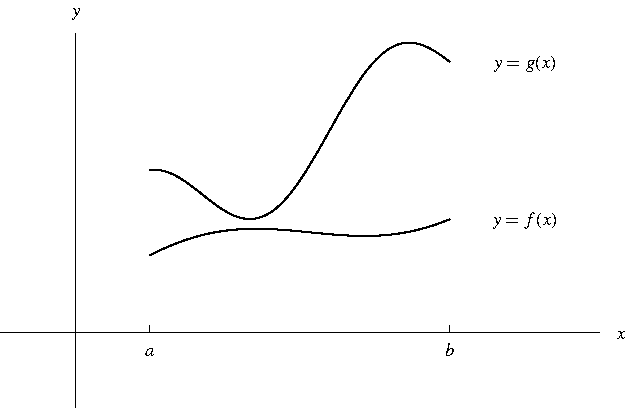
\includegraphics[height=4.2cm]{integration/pictures/05-02-comparisona.pdf}%
%}%
%\only<handout:0| 2>{%
%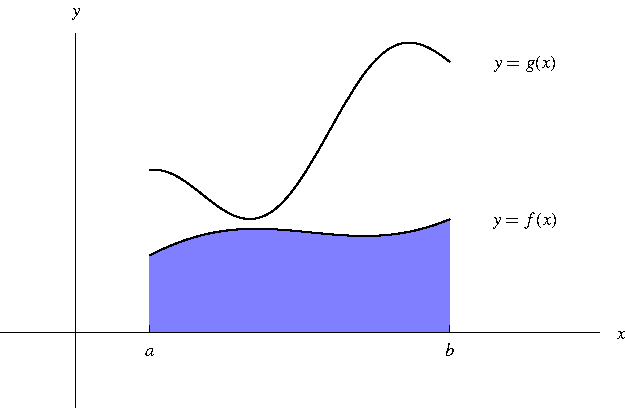
\includegraphics[height=4.2cm]{integration/pictures/05-02-comparisonb.pdf}%
%}%
%\only<handout:0| 3>{%
%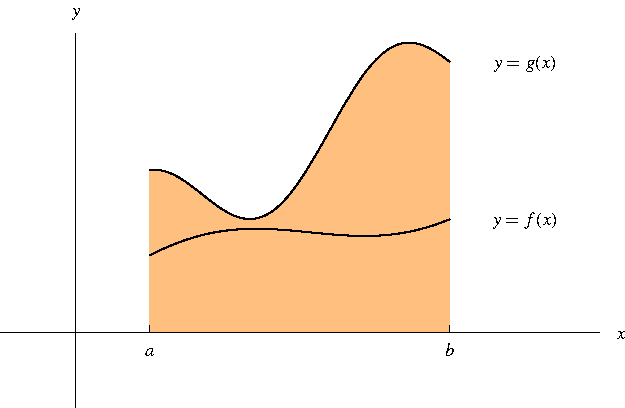
\includegraphics[height=4.2cm]{integration/pictures/05-02-comparisonc.pdf}%
%}%
\[
\alert<handout:0| 2>{\int_a^b f(x) \diff x}%
 \leq  %
\alert<handout:0| 3>{\int_a^b g(x) \diff x}%
\]
\end{center}
\end{frame}

\begin{frame}[t]
Comparison Properties of the Integral
\begin{enumerate}
\setcounter{enumi}{7}
\item  If $m\leq f(x)\leq M$ for all $a\leq x \leq b$, then
\[
\alert<handout:0| 2>{m(b-a)}%
 \leq  %
\alert<handout:0| 3>{\int_a^b f(x) \diff x}%
 \leq  %
\alert<handout:0| 4>{M(b-a)}%
\]
\end{enumerate}
\begin{center}
\psset{xunit=0.9cm, yunit=0.9cm}
\begin{pspicture}(-5, -5)(5,5)
\psframe*[linecolor=white](-5,-5)(5,5)
\psaxes[ticks=none, labels=none]{<->}(0,0)(-0.5,-0.5)(6,4.5)\tiny

\uncover<2>{
\pscustom*[linecolor=orange]{
\psplot[linecolor=\fcColorGraph, plotpoints=1000]{0.2}{5}{0.7}
\psline(5,0)(0.2,0)
}
}

\uncover<3>{
\pscustom*[linecolor=cyan!50]{
\psplot[linecolor=\fcColorGraph, plotpoints=1000]{0.2}{5}{x -9.9495 mul x 3 exp -2.0625 mul x 4 exp 0.1875 mul x 2 exp 7.4925 mul 5.6936 add add add add }
\psline(5,0)(0.2,0)
}
}
\uncover<4>{
\pscustom*[linecolor=cyan]{
\psplot[linecolor=red, plotpoints=1000]{0.2}{5}{4.3}
\psline(5,0)(0.2,0)
}
}
%Function formula: 7117/1250+2997/400 ((x)^{2})+3/16 ((x)^{4})-33/16 ((x)^{3})-19899/2000 (x)
\psplot[linecolor=\fcColorGraph, plotpoints=1000]{0.2}{5}{x -9.9495 mul x 3 exp -2.0625 mul x 4 exp 0.1875 mul x 2 exp 7.4925 mul 5.6936 add add add add }
\psline[linecolor=\fcColorGraph](0.2, 0.7)(5,0.7)
\psline[linecolor=\fcColorGraph](0.2, 4.3)(5, 4.3)


\rput[r](4.9, 2.6){\alert<3>{$y=f(x)$}}
\psline[linestyle=dotted, arrows=<->](5.05, 0)(5.05, 0.7)
\rput[l](5.15,0.35){\alert<2>{$m$}}
\psline[linestyle=dotted, arrows=<->](5.5, 0)(5.5, 4.3)
\rput[l](5.6,2.15){\alert<4>{$M$}}

\psline(0.2, -0.1)(0.2, 0.1)
\rput[t](0.2, -0.15){\alert<2,4>{$a$}}
\psline(5, -0.1)(5, 0.1)
\rput[t](5, -0.15){\alert<2,4>{$b$}}
\end{pspicture}
%\only<handout:0| -1>{%
%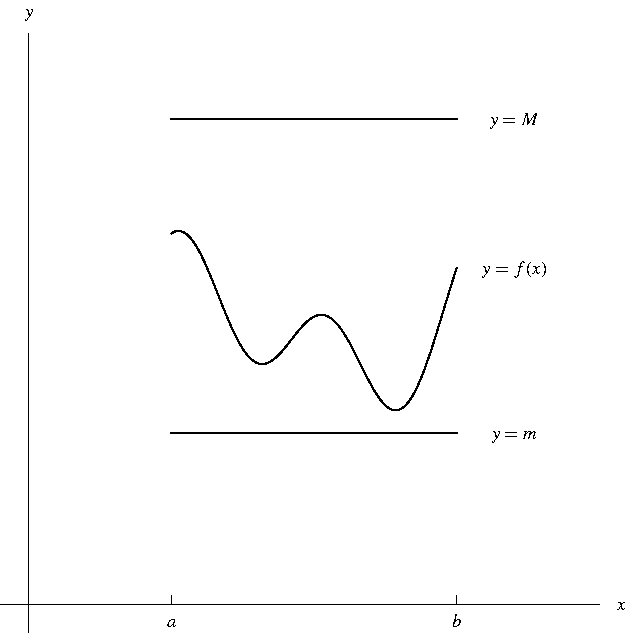
\includegraphics[height=5.6cm]{integration/pictures/05-02-boundinga.pdf}%
%}%
%\only<handout:0| 2>{%
%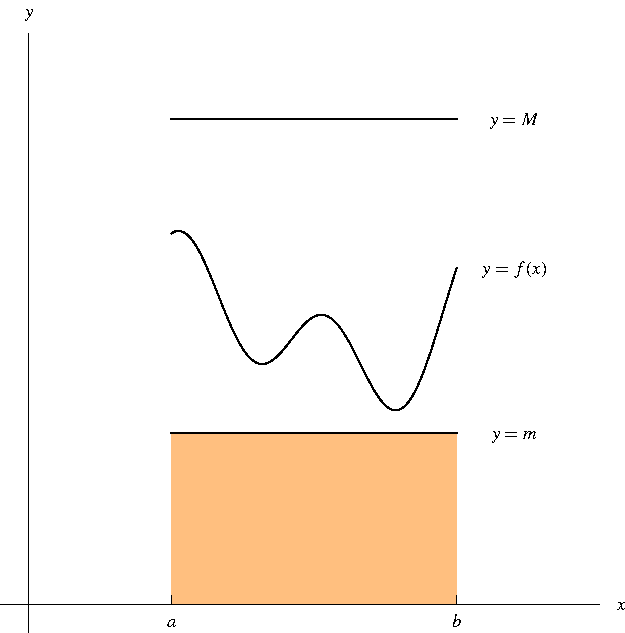
\includegraphics[height=5.6cm]{integration/pictures/05-02-boundingb.pdf}%
%}%
%\only<handout:0| 3>{%
%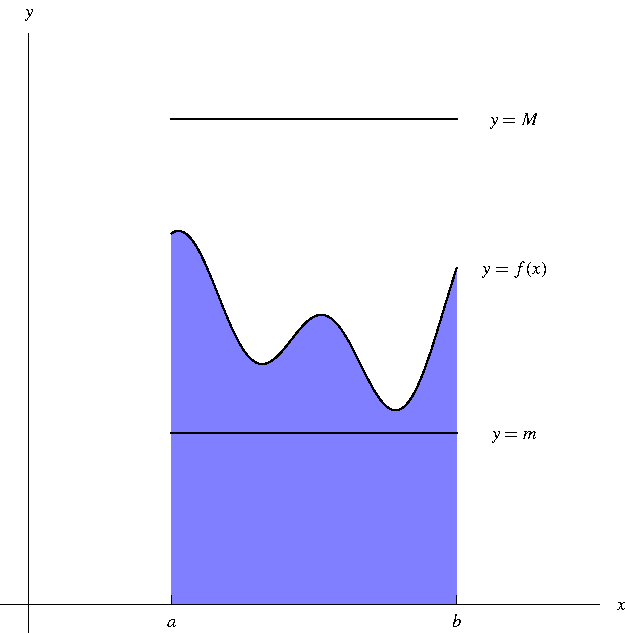
\includegraphics[height=5.6cm]{integration/pictures/05-02-boundingc.pdf}%
%}%
%\only<handout:0| 4>{%
%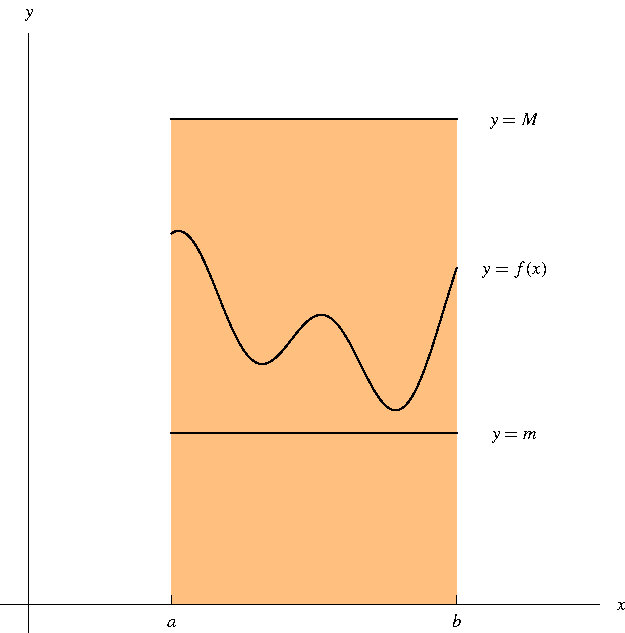
\includegraphics[height=5.6cm]{integration/pictures/05-02-boundingd.pdf}%
%}%
\end{center}
\end{frame}
% end module definite-integral-properties-comparison
